\documentclass{ltjsarticle} %lualatex cs_jikken.texで作成 
\usepackage{mdframed}
\usepackage{graphicx}
\usepackage{float}
\usepackage{array}
\usepackage{tikz}
\usepackage{circuitikz}
\usetikzlibrary{automata, positioning, arrows}
\begin{document}

\thispagestyle{empty}
\begin{flushright}
{\large 実験実施日 2024年11月7日,14日{\hspace{5cm}}} 
\end{flushright}

\vspace*{\fill}
\centering
{\Huge\bf コンピュータ科学実験b}
\vspace*{1cm}

{\huge\bf ソフトウェア実験 第1,2週レポート}
\vspace*{\fill}

\vspace*{\fill}

\vspace*{\fill}

\begin{flushright}
{\large 学生番号: 102210017} \\ % 5cmの空白を作り、アンダーラインを引く
{\large 氏名: 安藤 駿} \\

{\large 共同実験者: } \\
\end{flushright}

\clearpage

\addtocounter{page}{-1}
\raggedright
\setlength{\parindent}{1em}

\section{はじめに}
情報通信ネットワークは,現代の様々な計算機利用において必要不可欠のものとなっている.
本実験では, TCP/IP ネットワークにおける各種サービスの提供・利用のために必要な基本的知識を学習する
ことを目的とする. ローカルネットワーク・DMZネットワークを備えるサブネットネッ
トワークを構築し, Linux におけるネットワーク構成方法, ファイアウォールの設置方法について学習する.


\section{課題1 初期環境の確認}

\subsection{目的・概要}
各班用のルータmachine1の初期環境の確認をする。


\subsection{実験方法}

\subsubsection{中継用PCへのシリアル接続}
ネットワークインターフェイスが未設定な状態においては,ネット
ワーク経由の通信が不可能であることから, シリアル接続経由での通信を利用する必要がある. 
「ssh group00@icesc02」でmachine1にシリアル接続されたするための中継用PCにssh接続した. 
その後、「minicom group0.sh」でmachine1にシリアル接続した. 

\subsubsection{初期環境の確認}
「uname -r」で現在動作しているLinuxカーネルを確認した. 

「cat /etc/fstab」でファイルシステムのマウントポイントを記述した設定ファイル/etc/fstabの内容を確認した. 
「fdisk-l」でディスクパーティションを確認した. 
「df-h」でマウントされているファイルシステムを確認を確認した. 
「lvdisplay」で論理ボリュームの内容を確認した. 

「hostname icesc10.ice.nuie.nagoya-u.ac.jp」ででホスト名を設定し,
「hostname」で設定結果を確認した. 

「vi /etc/hostname」でvi エディタを用いて, ホスト名の恒久的変更をした. 
「exit」コマンドで script の終了後, 「reboot」コマンドで機器の再起動を行った. 

「cat /etc/sysconfig/selinux」,「getenforce」コマンドで, SELinux の設定状況の確認をした. 


\subsection{実験結果}
「uname -r」を実行すると「4.18.0-553.22.1.el8 10.x86 64」という結果が得られた. 

「cat /etc/fstab」を実行した結果を図\ref{fig:fstab}に示す. 
「fdisk -l」を実行した結果を図\ref{fig:fdisk}に示す. 
「df -h」を実行した結果を図\ref{fig:df}に示す. 
「lvdisplay」を実行した結果を図\ref{fig:lvdisplay}に示す. 

hostnameを設定した後「hostname」を実行すると, 「icesc10.ice.nuie.nagoya-u.ac.jp」という結果が得られた. 

「cat /etc/sysconfig/selinux」を実行した結果を図\ref{fig:selinux}に示す. 
「getenforce」を実行すると, 「Permissive」という結果が得られた. 

\begin{mdframed}
  \begin{verbatim}
#
# /etc/fstab
# Created by anaconda on Thu Oct 31 05:18:55 2024
#
# Accessible filesystems, by reference, are maintained under '/dev/disk/'.
# See man pages fstab(5), findfs(8), mount(8) and/or blkid(8) for more info.
#
# After editing this file, run 'systemctl daemon-reload' to update systemd
# units generated from this file.
#
/dev/mapper/cl-root     /                       xfs     defaults        0 0
UUID=308bebc3-bd1f-4724-a6b8-cb55e7d1a686 /boot                   xfs     defaul                                                                             ts        0 0
/dev/mapper/cl-home     /home                   xfs     defaults        0 0
/dev/mapper/cl-swap     none                    swap    defaults        0 0
  \end{verbatim}
  \end{mdframed}
  \begin{figure}[H]
  \caption{「cat /etc/fstab」の結果}
  \label{fig:fstab}
\end{figure}

\begin{mdframed}
  \begin{verbatim}
Disk /dev/sda: 232.9 GiB, 250059350016 bytes, 488397168 sectors
Units: sectors of 1 * 512 = 512 bytes  
Sector size (logical/physical): 512 bytes / 512 bytes  
I/O size (minimum/optimal): 512 bytes / 512 bytes  
Disklabel type: dos  
Disk identifier: 0x493d6230
Device     Boot   Start       End   Sectors   Size Id Type
/dev/sda1  *       2048   2099199   2097152     1G 83 Linux
/dev/sda2       2099200 488396799 486297600 231.9G 8e Linux LVM

Disk /dev/mapper/cl-root: 50 GiB, 53687091200 bytes, 104857600 sectors
Units: sectors of 1 * 512 = 512 bytes
Sector size (logical/physical): 512 bytes / 512 bytes
I/O size (minimum/optimal): 512 bytes / 512 bytes

Disk /dev/mapper/cl-swap: 8 GiB, 8589934592 bytes, 16777216 sectors
Units: sectors of 1 * 512 = 512 bytes
Sector size (logical/physical): 512 bytes / 512 bytes
I/O size (minimum/optimal): 512 bytes / 512 bytes

Disk /dev/mapper/cl-home: 173.9 GiB, 186705248256 bytes, 364658688 sectors
Units: sectors of 1 * 512 = 512 bytes
Sector size (logical/physical): 512 bytes / 512 bytes
I/O size (minimum/optimal): 512 bytes / 512 bytes
  \end{verbatim}
  \end{mdframed}
  \begin{figure}[H]
  \caption{「fdisk -l」の結果}
  \label{fig:fdisk}
\end{figure}

\begin{mdframed}
  \begin{verbatim}
  Filesystem           Size  Used Avail Use% Mounted on
  devtmpfs             3.7G     0  3.7G   0% /dev
  tmpfs                3.8G     0  3.8G   0% /dev/shm
  tmpfs                3.8G   41M  3.7G   2% /run
  tmpfs                3.8G     0  3.8G   0% /sys/fs/cgroup
  /dev/mapper/cl-root   50G  2.4G   48G   5% /
  /dev/sda1           1014M  237M  778M  24% /boot
  /dev/mapper/cl-home  174G  1.3G  173G   1% /home
  tmpfs                759M     0  759M   0% /run/user/0
  \end{verbatim}
  \end{mdframed}
  \begin{figure}[H]
  \caption{「df -h」の結果}
  \label{fig:df}
\end{figure}

\begin{mdframed}
  \begin{verbatim}
--- Logical volume ---
LV Path                /dev/cl/root
LV Name                root
VG Name                cl
LV UUID                2dWUBg-dzsa-C0wC-KAJr-SRqB-AJVi-pcRSf5
LV Write Access        read/write
LV Creation host, time localhost.localdomain, 2024-10-31 14:18:48 +0900
LV Status              available
# open                 1
LV Size                50.00 GiB
Current LE             12800
Segments               1
Allocation             inherit
Read ahead sectors     auto
- currently set to     8192
Block device           253:0

--- Logical volume ---
LV Path                /dev/cl/swap
LV Name                swap
VG Name                cl
LV UUID                9Tb02T-cVXq-Cfgb-z1y8-aJn2-QpuP-9x2a2G
LV Write Access        read/write
LV Creation host, time localhost.localdomain, 2024-10-31 14:18:48 +0900
LV Status              available
# open                 2
LV Size                8.00 GiB
Current LE             2048
Segments               1
Allocation             inherit
Read ahead sectors     auto
- currently set to     8192
Block device           253:1

--- Logical volume ---
LV Path                /dev/cl/home
LV Name                home
VG Name                cl
LV UUID                6APbSp-1DIq-RBs4-xA6z-QfqT-bfv9-75QzSQ
LV Write Access        read/write
LV Creation host, time localhost.localdomain, 2024-10-31 14:18:49 +0900
LV Status              available
# open                 1
LV Size                173.88 GiB
Current LE             44514
Segments               1
Allocation             inherit
Read ahead sectors     auto
- currently set to     8192
Block device           253:2
  \end{verbatim}
  \end{mdframed}
  \begin{figure}[H]
  \caption{「lvdisplay」の結果}
  \label{fig:lvdisplay}
\end{figure}

\begin{mdframed}
  \begin{verbatim}
# This file controls the state of SELinux on the system.
# SELINUX= can take one of these three values:
#     enforcing - SELinux security policy is enforced.
#     permissive - SELinux prints warnings instead of enforcing.
#     disabled - No SELinux policy is loaded.
SELINUX=permissive
# SELINUXTYPE= can take one of these three values:
#     targeted - Targeted processes are protected,
#     minimum - Modification of targeted policy. Only selected processes are protected.
#     mls - Multi Level Security protection.
SELINUXTYPE=targeted
  \end{verbatim}
  \end{mdframed}
  \begin{figure}[H]
  \caption{「cat /etc/sysconfig/selinux」の結果}
  \label{fig:selinux}
\end{figure}

\subsection{考察}
「uname -r」の結果「4.18.0-553.22.1.el8 10.x86 64」から, Linux カーネルのバージョンが 4.18.0であり, 
カーネルのリリース番号が553.22.1で, RHEL 8(またはそのクローン)用にビルドされており, 
64ビット アーキテクチャ(x86 64)用であることが分かる. 

「cat /etc/fstab」の結果から,  /dev/mapper/cl-rootのマウントポイントが/, ファイルシステムの種類がxfs
オプションがdefaults, バックアップオプションが0, ファイルシステムチェックオプションが0であることが分かる. 
UUID=308bebc3-bd1f-4724-a6b8-cb55e7d1a686から, マウントポイントが/bootであることが分かる. 
/dev/mapper/cl-homeから, マウントポイントが/homeであることが分かる. 
/dev/mapper/cl-swapから, マウントポイントがnone, ファイルシステムの種類がswapであることが分かる. 

「fdisk -l」の結果から, /dev/sda は、232.9GBのディスクで, /dev/sda1(1GB)は通常のLinuxパーティション, 
/dev/sda2(231.9GB)はLVM用のパーティションであると考えられる.  
LVMの論理ボリュームには, /dev/mapper/cl-root, /dev/mapper/cl-swap, 
/dev/mapper/cl-homeが含まれていることが分かる. 
この構成では, LVMを使用して柔軟なパーティション管理が行われており, 物理ディスク(/dev/sda)に対して論理ボリュームを作成していると考えられる. 

「df -h」の結果から, システムのファイルシステムのディスク使用状況を確認できる. 
各ファイルシステムについて, サイズ, 使用済み容量, 空き容量, 使用率, マウントポイントが分かる. 

「lvdisplay」の結果から, 現在のシステムにおける論理ボリューム(LVM)の状態が確認できる. 
各論理ボリュームについて, LV名, VG名: cl(ボリュームグループ名), LVサイズ, 現在のLE数, 
状態, ブロックデバイス, アクセス方法, 作成日時, オープン状態, リードアヘッドセクタ数が分かる. 

「cat /etc/sysconfig/selinux」の結果から, SELinuxの状態はpermissiveであり, SELinuxは警告を表示するが, 
強制的な制限は行っていない状態であることが分かる. 
SELinuxのポリシータイプはtargetedであり, セキュリティポリシーは特定の重要なプロセスにのみ適用される設定となっていることが分かる. 

\section{課題2 ネットワーク設定}

\subsection{目的・概要}
machine1において, nmcliコマンドを利用して, ネットワークインターフェイスの接続設定を行う.

\subsection{実験方法}

\subsubsection{初期状況の確認}
「nmcli device status」で接続されているネットワークデバイスの現在の状態を確認し, 
「nmcli device show」でシステム内のネットワークデバイスに関する詳細情報を確認した. 

「nmcli connection show」でネットワーク接続の確認をした. 

\subsubsection{接続設定の修正}
「nmcli con show enp1s0」でLAN1の現在の設定値を確認した. 
「nmcli con mod enp1s0 ipv4.method manual ipv4.addr "192.168.100.10/24"」で, 
IPv4 の method をmanualに変更し, アドレスを 192.168.100.10, ネットマスクを /24に設定した. 
「nmcli con mod enp1s0 ipv4.dns "10.10.1.2"」でDNS サーバーの IP アドレスを設定した. 
「nmcli con mod enp1s0 ipv4.dns-search "ice.nuie.nagoya-u.ac.jp"」でDNS 検索ドメインを設定した. 
「nmcli con mod enp1s0 ipv4.gateway "192.168.100.1"」でデフォルトゲートウェイを設定した. 
「nmcli con mod enp1s0 connection.autoconnect "yes"」 で 自動接続を設定した. 
再び「nmcli con show enp1s0」を実行し, 変更が反映されているかを確認した. 

「nmcli con mod enp2s0 ipv4.method manual ipv4.addr "192.168.150.1/24"」でLAN2の
IPv4 の method をmanualに変更し, アドレスを 192.168.150.1, ネットマスクを /24に設定した. 
「nmcli con show enp2s0」を実行し, 変更が反映されているかを確認した.

「nmcli con mod enp3s0 ipv4.method manual ipv4.addr "192.168.200.1/24"」でLAN3の
IPv4 の method をmanualに変更し, アドレスを 192.168.200.1, ネットマスクを /24に設定した. 
「nmcli con show enp3s0」を実行し, 変更が反映されているかを確認した. 

再び「nmcli dev status」を実行し, 接続されているネットワークデバイスの現在の状態を確認し, 
「nmcli con show」でシステム内のネットワークデバイスに関する詳細情報を確認した. 

\subsubsection{各種情報の再確認}
「ip addr show」で各デバイスの設定の確認をした. 
「ip route」でルーティング情報の確認をした. 
「cat /etc/resolv.conf」でDNS設定の確認をした. 

\subsection{実験結果}

\subsubsection{初期状況の確認}
「nmcli device status」を実行した結果を図\ref{fig:status}に示す. 
「nmcli device show」を実行した結果を図\ref{fig:show}に示す. 
「nmcli connection show」を実行した結果を\ref{fig:con_show}に示す. 

\begin{mdframed}
  \begin{verbatim}
  DEVICE  TYPE      STATE         CONNECTION
  enp1s0  ethernet  disconnected  --
  enp2s0  ethernet  disconnected  --
  enp3s0  ethernet  disconnected  --
  enp4s0  ethernet  unavailable   --
  lo      loopback  unmanaged     --
  \end{verbatim}
  \end{mdframed}
  \begin{figure}[H]
  \caption{「nmcli device status」の結果}
  \label{fig:status}
\end{figure}

\begin{mdframed}
  \begin{verbatim}
GENERAL.DEVICE:                         enp1s0
GENERAL.TYPE:                           ethernet
GENERAL.HWADDR:                         00:E0:67:12:2D:BC
GENERAL.MTU:                            1500
GENERAL.STATE:                          30 (disconnected)
GENERAL.CONNECTION:                     --
GENERAL.CON-PATH:                       --
WIRED-PROPERTIES.CARRIER:               on
IP4.GATEWAY:                            --
IP6.GATEWAY:                            --

GENERAL.DEVICE:                         enp2s0
GENERAL.TYPE:                           ethernet
GENERAL.HWADDR:                         00:E0:67:12:2D:BD
GENERAL.MTU:                            1500
GENERAL.STATE:                          30 (disconnected)
GENERAL.CONNECTION:                     --
GENERAL.CON-PATH:                       --
WIRED-PROPERTIES.CARRIER:               on
IP4.GATEWAY:                            --
IP6.GATEWAY:                            --

GENERAL.DEVICE:                         enp3s0
GENERAL.TYPE:                           ethernet
GENERAL.HWADDR:                         00:E0:67:12:2D:BE
GENERAL.MTU:                            1500
GENERAL.STATE:                          30 (disconnected)
GENERAL.CONNECTION:                     --
GENERAL.CON-PATH:                       --
WIRED-PROPERTIES.CARRIER:               on
IP4.GATEWAY:                            --
IP6.GATEWAY:                            --

GENERAL.DEVICE:                         enp4s0
GENERAL.TYPE:                           ethernet
GENERAL.HWADDR:                         00:E0:67:12:2D:BF
GENERAL.MTU:                            1500
GENERAL.STATE:                          20 (unavailable)
GENERAL.CONNECTION:                     --
GENERAL.CON-PATH:                       --
WIRED-PROPERTIES.CARRIER:               off
IP4.GATEWAY:                            --
IP6.GATEWAY:                            --

GENERAL.DEVICE:                         lo
GENERAL.TYPE:                           loopback
GENERAL.HWADDR:                         00:00:00:00:00:00
GENERAL.MTU:                            65536
GENERAL.STATE:                          10 (unmanaged)
GENERAL.CONNECTION:                     --
GENERAL.CON-PATH:                       --
IP4.ADDRESS[1]:                         127.0.0.1/8
IP4.GATEWAY:                            --
IP6.ADDRESS[1]:                         ::1/128
IP6.GATEWAY:                            --
IP6.ROUTE[1]:                           dst = ::1/128, nh = ::, mt = 256
  \end{verbatim}
  \end{mdframed}
  \begin{figure}[H]
  \caption{「nmcli device show」の結果}
  \label{fig:show}
\end{figure}

\begin{mdframed}
  \begin{verbatim}
NAME    UUID                                  TYPE      DEVICE
enp1s0  36f99f9b-fb0e-419f-aa68-01de0c4a37d9  ethernet  enp1s0
enp2s0  69fa7f59-f490-4a80-ada3-f5156e3f2a82  ethernet  --
enp3s0  f49e9852-ad73-4316-a476-f85183f03b72  ethernet  --
enp4s0  61d32de9-4582-4208-ba06-c9cba2021ff0  ethernet  --
  \end{verbatim}
  \end{mdframed}
  \begin{figure}[H]
  \caption{「nmcli connection show」の結果}
  \label{fig:con_show}
\end{figure}

\subsubsection{接続設定の修正}
LAN1の設定値を変更後「nmcli con show enp1s0」を実行した結果を図\ref{fig:enp1s0}に, 
LAN2の設定値を変更後「nmcli con show enp2s0」を実行した結果を図\ref{fig:enp2s0}に,  
LAN3の設定値を変更後「nmcli con show enp3s0」を実行した結果を図\ref{fig:enp3s0}に示す. 

再び「nmcli dev status」を実行した結果を図\ref{fig:status2}に, 
「nmcli con show」を実行した結果を図\ref{fig:con_show2}に示す. 


\begin{mdframed}
  \begin{verbatim}
connection.id:                          enp1s0
connection.uuid:                        36f99f9b-fb0e-419f-aa68-01de0c4a37d9
connection.stable-id:                   --
connection.type:                        802-3-ethernet
connection.interface-name:              enp1s0
connection.autoconnect:                 はい
connection.autoconnect-priority:        -100
connection.autoconnect-retries:         1
connection.multi-connect:               0 (default)
connection.auth-retries:                -1
connection.timestamp:                   1730959861
connection.read-only:                   いいえ
connection.permissions:                 --
connection.zone:                        --
connection.master:                      --
connection.slave-type:                  --
connection.autoconnect-slaves:          -1 (default)
connection.secondaries:                 --
connection.gateway-ping-timeout:        0
connection.metered:                     不明
connection.lldp:                        default
connection.mdns:                        -1 (default)
connection.llmnr:                       -1 (default)
connection.dns-over-tls:                -1 (default)
connection.mptcp-flags:                 0x0 (default)
connection.wait-device-timeout:         -1
connection.wait-activation-delay:       -1

  --省略--
  
ipv4.method:                            manual
ipv4.dns:                               10.10.1.2
ipv4.dns-search:                        ice.nuie.nagoya-u.ac.jp
ipv4.dns-options:                       --
ipv4.dns-priority:                      0
ipv4.addresses:                         192.168.100.10/24
ipv4.gateway:                           192.168.100.1
ipv4.routes:                            --
ipv4.route-metric:                      -1
ipv4.route-table:                       0 (unspec)
ipv4.routing-rules:                     --
ipv4.ignore-auto-routes:                いいえ
ipv4.ignore-auto-dns:                   いいえ
ipv4.dhcp-client-id:                    --
ipv4.dhcp-iaid:                         --
ipv4.dhcp-timeout:                      90
ipv4.dhcp-send-hostname:                はい
ipv4.dhcp-hostname:                     --
ipv4.dhcp-fqdn:                         --
ipv4.dhcp-hostname-flags:               0x0 (none)
ipv4.never-default:                     いいえ
ipv4.may-fail:                          いいえ
ipv4.required-timeout:                  -1 (default)
ipv4.dad-timeout:                       -1 (default)
ipv4.dhcp-vendor-class-identifier:      anaconda-Linux
ipv4.link-local:                        0 (default)
ipv4.dhcp-reject-servers:               --
  
  --省略--

IP4.ADDRESS[1]:                         192.168.100.10/24
IP4.GATEWAY:                            192.168.100.1
IP4.ROUTE[1]:                           dst = 192.168.100.0/24, nh = 0.0.0.0, mt = 100
IP4.ROUTE[2]:                           dst = 0.0.0.0/0, nh = 192.168.100.1, mt = 100
IP4.DNS[1]:                             10.10.1.2
IP4.SEARCHES[1]:                        ice.nuie.nagoya-u.ac.jp
IP6.ADDRESS[1]:                         fe80::2e0:67ff:fe12:2dbc/64
IP6.GATEWAY:                            --
IP6.ROUTE[1]:                           dst = fe80::/64, nh = ::, mt = 1024
  \end{verbatim}
  \end{mdframed}
  \begin{figure}[H]
  \caption{「nmcli con show enp1s0」の結果の一部}
  \label{fig:enp1s0}
\end{figure}

\begin{mdframed}
  \begin{verbatim}
connection.id:                          enp2s0
connection.uuid:                        69fa7f59-f490-4a80-ada3-f5156e3f2a82
connection.stable-id:                   --
connection.type:                        802-3-ethernet
connection.interface-name:              enp2s0
connection.autoconnect:                 はい
connection.autoconnect-priority:        0
connection.autoconnect-retries:         -1 (default)
connection.multi-connect:               0 (default)
connection.auth-retries:                -1
connection.timestamp:                   1730964562
connection.read-only:                   いいえ
connection.permissions:                 --
connection.zone:                        --
connection.master:                      --
connection.slave-type:                  --
connection.autoconnect-slaves:          -1 (default)
connection.secondaries:                 --
connection.gateway-ping-timeout:        0
connection.metered:                     不明
connection.lldp:                        default
connection.mdns:                        -1 (default)
connection.llmnr:                       -1 (default)
connection.dns-over-tls:                -1 (default)
connection.mptcp-flags:                 0x0 (default)
connection.wait-device-timeout:         -1
connection.wait-activation-delay:       -1
  
  --省略--

ipv4.method:                            manual
ipv4.dns:                               --
ipv4.dns-search:                        --
ipv4.dns-options:                       --
ipv4.dns-priority:                      0
ipv4.addresses:                         192.168.150.1/24
ipv4.gateway:                           --
ipv4.routes:                            --
ipv4.route-metric:                      -1
ipv4.route-table:                       0 (unspec)
ipv4.routing-rules:                     --
ipv4.ignore-auto-routes:                いいえ
ipv4.ignore-auto-dns:                   いいえ
ipv4.dhcp-client-id:                    --
ipv4.dhcp-iaid:                         --
ipv4.dhcp-timeout:                      0 (default)
ipv4.dhcp-send-hostname:                はい
ipv4.dhcp-hostname:                     --
ipv4.dhcp-fqdn:                         --
ipv4.dhcp-hostname-flags:               0x0 (none)
ipv4.never-default:                     いいえ
ipv4.may-fail:                          はい
ipv4.required-timeout:                  -1 (default)
ipv4.dad-timeout:                       -1 (default)
ipv4.dhcp-vendor-class-identifier:      --
ipv4.link-local:                        0 (default)
ipv4.dhcp-reject-servers:               --

  --省略--

IP4.ADDRESS[1]:                         192.168.150.1/24
IP4.GATEWAY:                            --
IP4.ROUTE[1]:                           dst = 192.168.150.0/24, nh = 0.0.0.0, mt = 103
IP6.ADDRESS[1]:                         fe80::2e0:67ff:fe12:2dbd/64
IP6.GATEWAY:                            --
IP6.ROUTE[1]:                           dst = fe80::/64, nh = ::, mt = 1024
  \end{verbatim}
  \end{mdframed}
  \begin{figure}[H]
  \caption{「nmcli con show enp2s0」の結果の一部}
  \label{fig:enp2s0}
\end{figure}

\begin{mdframed}
  \begin{verbatim}
connection.id:                          enp3s0
connection.uuid:                        f49e9852-ad73-4316-a476-f85183f03b72
connection.stable-id:                   --
connection.type:                        802-3-ethernet
connection.interface-name:              enp3s0
connection.autoconnect:                 はい
connection.autoconnect-priority:        0
connection.autoconnect-retries:         -1 (default)
connection.multi-connect:               0 (default)
connection.auth-retries:                -1
connection.timestamp:                   1730959863
connection.read-only:                   いいえ
connection.permissions:                 --
connection.zone:                        --
connection.master:                      --
connection.slave-type:                  --
connection.autoconnect-slaves:          -1 (default)
connection.secondaries:                 --
connection.gateway-ping-timeout:        0
connection.metered:                     不明
connection.lldp:                        default
connection.mdns:                        -1 (default)
connection.llmnr:                       -1 (default)
connection.dns-over-tls:                -1 (default)
connection.mptcp-flags:                 0x0 (default)
connection.wait-device-timeout:         -1
connection.wait-activation-delay:       -1

  --省略--

ipv4.method:                            manual
ipv4.dns:                               --
ipv4.dns-search:                        --
ipv4.dns-options:                       --
ipv4.dns-priority:                      0
ipv4.addresses:                         192.168.200.1/24
ipv4.gateway:                           --
ipv4.routes:                            --
ipv4.route-metric:                      -1
ipv4.route-table:                       0 (unspec)
ipv4.routing-rules:                     --
ipv4.ignore-auto-routes:                いいえ
ipv4.ignore-auto-dns:                   いいえ
ipv4.dhcp-client-id:                    --
ipv4.dhcp-iaid:                         --
ipv4.dhcp-timeout:                      0 (default)
ipv4.dhcp-send-hostname:                はい
ipv4.dhcp-hostname:                     --
ipv4.dhcp-fqdn:                         --
ipv4.dhcp-hostname-flags:               0x0 (none)
ipv4.never-default:                     いいえ
ipv4.may-fail:                          はい
ipv4.required-timeout:                  -1 (default)
ipv4.dad-timeout:                       -1 (default)
ipv4.dhcp-vendor-class-identifier:      --
ipv4.link-local:                        0 (default)
ipv4.dhcp-reject-servers:               --

  --省略--

IP4.ADDRESS[1]:                         192.168.200.1/24
IP4.GATEWAY:                            --
IP4.ROUTE[1]:                           dst = 192.168.200.0/24, nh = 0.0.0.0, mt = 102
IP6.ADDRESS[1]:                         fe80::2e0:67ff:fe12:2dbe/64
IP6.GATEWAY:                            --
IP6.ROUTE[1]:                           dst = fe80::/64, nh = ::, mt = 1024
  \end{verbatim}
  \end{mdframed}
  \begin{figure}[H]
  \caption{「nmcli con show enp3s0」の結果の一部}
  \label{fig:enp3s0}
\end{figure}

\begin{mdframed}
  \begin{verbatim}
  DEVICE  TYPE      STATE        CONNECTION
  enp1s0  ethernet  connected    enp1s0
  enp2s0  ethernet  connected    enp2s0
  enp3s0  ethernet  connected    enp3s0
  enp4s0  ethernet  unavailable  --
  lo      loopback  unmanaged    --
  \end{verbatim}
  \end{mdframed}
  \begin{figure}[H]
  \caption{「nmcli dev status」の結果}
  \label{fig:status2}
\end{figure}

\begin{mdframed}
  \begin{verbatim}
NAME    UUID                                  TYPE      DEVICE
enp1s0  36f99f9b-fb0e-419f-aa68-01de0c4a37d9  ethernet  enp1s0
enp2s0  69fa7f59-f490-4a80-ada3-f5156e3f2a82  ethernet  enp2s0
enp3s0  f49e9852-ad73-4316-a476-f85183f03b72  ethernet  enp3s0
enp4s0  61d32de9-4582-4208-ba06-c9cba2021ff0  ethernet  --
  \end{verbatim}
  \end{mdframed}
  \begin{figure}[H]
  \caption{「nmcli con show」の結果}
  \label{fig:con_show2}
\end{figure}


\subsubsection{各種情報の再確認}
「ip addr show」の実行結果を図\ref{fig:addr_show}に, 
「ip route」の実行結果を図\ref{fig:route}に,
「cat /etc/resolv.conf」の実行結果を図\ref{fig:resolv}に示す. 

\begin{mdframed}
  \begin{verbatim}
1: lo: <LOOPBACK,UP,LOWER_UP> mtu 65536 qdisc noqueue state UNKNOWN group default qlen 1000
    link/loopback 00:00:00:00:00:00 brd 00:00:00:00:00:00
    inet 127.0.0.1/8 scope host lo
      valid_lft forever preferred_lft forever
    inet6 ::1/128 scope host
      valid_lft forever preferred_lft forever
2: enp1s0: <BROADCAST,MULTICAST,UP,LOWER_UP> mtu 1500 qdisc fq_codel state UP group default qlen 1000
    link/ether 00:e0:67:12:2d:bc brd ff:ff:ff:ff:ff:ff
    inet 192.168.100.10/24 brd 192.168.100.255 scope global noprefixroute enp1s0
      valid_lft forever preferred_lft forever
    inet6 fe80::2e0:67ff:fe12:2dbc/64 scope link noprefixroute
      valid_lft forever preferred_lft forever
3: enp2s0: <BROADCAST,MULTICAST,UP,LOWER_UP> mtu 1500 qdisc fq_codel state UP group default qlen 1000
    link/ether 00:e0:67:12:2d:bd brd ff:ff:ff:ff:ff:ff
    inet 192.168.150.1/24 brd 192.168.150.255 scope global noprefixroute enp2s0
      valid_lft forever preferred_lft forever
    inet6 fe80::2e0:67ff:fe12:2dbd/64 scope link noprefixroute
      valid_lft forever preferred_lft forever
4: enp3s0: <BROADCAST,MULTICAST,UP,LOWER_UP> mtu 1500 qdisc fq_codel state UP group default qlen 1000
    link/ether 00:e0:67:12:2d:be brd ff:ff:ff:ff:ff:ff
    inet 192.168.200.1/24 brd 192.168.200.255 scope global noprefixroute enp3s0
      valid_lft forever preferred_lft forever
    inet6 fe80::2e0:67ff:fe12:2dbe/64 scope link noprefixroute
      valid_lft forever preferred_lft forever
5: enp4s0: <NO-CARRIER,BROADCAST,MULTICAST,UP> mtu 1500 qdisc fq_codel state DOWN group default qlen 1000
    link/ether 00:e0:67:12:2d:bf brd ff:ff:ff:ff:ff:ff
  \end{verbatim}
  \end{mdframed}
  \begin{figure}[H]
  \caption{「ip addr show」の結果}
  \label{fig:addr_show}
\end{figure}

\begin{mdframed}
  \begin{verbatim}
default via 192.168.100.1 dev enp1s0 proto static metric 103
192.168.100.0/24 dev enp1s0 proto kernel scope link src 192.168.100.10 metric 103
192.168.150.0/24 dev enp2s0 proto kernel scope link src 192.168.150.1 metric 101
192.168.200.0/24 dev enp3s0 proto kernel scope link src 192.168.200.1 metric 102
  \end{verbatim}
  \end{mdframed}
  \begin{figure}[H]
  \caption{「ip route」の結果}
  \label{fig:route}
\end{figure}

\begin{mdframed}
  \begin{verbatim}
  # Generated by NetworkManager
  search ice.nuie.nagoya-u.ac.jp
  nameserver 10.10.1.2
  \end{verbatim}
  \end{mdframed}
  \begin{figure}[H]
  \caption{「cat /etc/resolv.conf」の結果}
  \label{fig:resolv}
\end{figure}

\subsection{考察}

\subsubsection{初期状況の確認}
「nmcli device status」の結果から, enp1s0, enp2s0, enp3s0 はすべて disconnected 状態にあり, 
これらの Ethernet インターフェースは物理的に接続されていないか, ネットワーク接続が確立されていない状態であると考えられる. 

「nmcli connection show」の結果から, 各ネットワークインターフェースの詳細情報を確認することができる. 
HWADDRはこれはネットワークインターフェースのMACアドレスを示しており, 
MTUは1回の転送で送信できる最大のデータパケットサイズを示しており, 
STATEはこのインターフェースは状態を示しており, 
CARRIERは物理的な接続の有無を示しており, 
IP4.GATEWAY, IP6.GATEWAYはIPv4およびIPv6のゲートウェイ情報を示している. 
各Ethernetインターフェースはすべて接続されていないか利用できない状態であることが分かる. 

「nmcli con show」の結果から, ネットワークインターフェースの接続状態についていくつかの情報を得ることができる. 
UUIDは各ネットワークインターフェースに一意の識別子(UUID)を示しており, 
TYPEはインターフェースの種類を示しており, DEVICEはデバイス名を示している. 

\subsubsection{接続設定の修正}
LAN1の設定値を変更後「nmcli con show enp1s0」を実行した結果より, LAN1 の ipv4.method を manualに, 
ipv4.addr を 192.168.100.10/24 に,  ipv4.dns を 10.10.1.2 に,  ipv4.dns-search を 
ice.nuie.nagoya-u.ac.jp に, ipv4.gateway を 192.168.100.1 に, 
connection.autoconnect を yes に設定できていると判断できる. 

LAN2の設定値を変更後「nmcli con show enp2s0」を実行した結果より, LAN2 の ipv4.method を manualに, 
ipv4.addr を 192.168.150.1/24 に設定できていると判断できる. 

LAN3の設定値を変更後「nmcli con show enp3s0」を実行した結果より, LAN3 の ipv4.method を manualに, 
ipv4.addr を 192.168.200.1/24 に設定できていると判断できる.

「nmclidevstatus」, 「nmcliconshow」の結果から, enp1s0, enp2s0, enp3s0 は正常にネットワークに接続されたと考えられる. 

\subsubsection{各種情報の再確認}
「ip addr show」の結果から, enp1s0, enp2s0, enp3s0 はそれぞれ異なるサブネット(192.168.100.10, 192.168.150.1, 192.168.200.1)
に接続されたネットワークインターフェースであると判断できる. 
enp4s0 は物理的に接続されていない状態で、現在は利用できないことが分かる. 

「ip route」の結果から, 192.168.100.0/24、192.168.150.0/24、192.168.200.0/24 の
各ネットワークに対するルートが, それぞれ enp1s0、enp2s0、enp3s0 インターフェースを経由して設定されており, 
enp1s0には192.168.100.10, enp2s0には192.168.150.1, enp3s0には192.168.200.1がIPアドレスとして設定されていることが分かる. 

「cat /etc/resolv.conf」の結果から, 検索ドメインがice.nuie.nagoya-u.ac.jpであること, 
DNSサーバーが10.10.1.2であることが分かる. 

これらのことから, machine1 の ネットワークインターフェイスの接続設定を正しく実施することができたと判断できる.  

\section{課題3 DHCPサービスの設定・起動}

\subsection{目的・概要}
machine1でDHCPサーバを動作させ, DMZネットワークと各班用ネットワークの両方のサブ
ネット接続機器への設定情報の提供を行う.

\subsection{実験方法}

\subsubsection{firewall の停止}
「systemctl stop firewalld」で一時的にfirewallを停止した. 
「systemctl status firewalld」でstatus が inactive となっていることを確認した. 

\subsubsection{DHCPサーバのインストールと設定}
「yum list dhcp-*」,「yum info dhcp-server」,「yum install dhcp-server」で
DHCP関連パッケージの確認とDHCPサーバのインストールをした. 

「vi /etc/dhcp/dhcpd.conf」でdhcpd.confを図\ref{fig:dhcpd_conf}のように編集した. 

「systemctl start dhcpd」でDHCPサーバを起動した. 
「systemctl status dhcpd」でDHCPサーバの状態がactive(動作中)であることを確認した. 
「systemctl enable dhcpd」でDHCPサーバのブート時自動起動を指定した. 

「ping 192.168.150.2」,「ping 192.168.200.100」でmachine2, machine3の生存を確認した. 

machine2, machine3にsshでログインし, 「ip addr show」,「ip route」,「cat /etc/resolv.conf」
を実行し, ネットワーク設定が行われていることを確認した. 

\begin{mdframed}
  \begin{verbatim}
#
# DHCP Server Configuration file.
#   see /usr/share/doc/dhcp-server/dhcpd.conf.example
#   see dhcpd.conf(5) man page

default-lease-time 3600;
max-lease-time 86400;
subnet 192.168.150.0 netmask 255.255.255.0 {
  range 192.168.150.100 192.168.150.250;
  option routers 192.168.150.1;
  option domain-name-servers 10.10.1.2;
  option domain-name "ice.nuie.nagoya-u.ac.jp";
}
host www0 {
  hardware ethernet 94:c6:91:a9:0c:0e;
  fixed-address 192.168.150.2;
  default-lease-time 2592000;
  max-lease-time 2592000;
}
subnet 192.168.200.0 netmask 255.255.255.0 {
  range 192.168.200.100 192.168.200.250;
  option routers 192.168.200.1;
  option domain-name-servers 10.10.1.2;
  option domain-name "ice.nuie.nagoya-u.ac.jp";
}
  \end{verbatim}
  \end{mdframed}
  \begin{figure}[H]
  \caption{dhcpd.conf}
  \label{fig:dhcpd_conf}
\end{figure}


\subsection{実験結果}

\subsubsection{firewall の停止}
「systemctl status firewalld」を実行した結果を図\ref{fig:firewall}に示す. 

\begin{mdframed}
  \begin{verbatim}
firewalld.service - firewalld - dynamic firewall daemon
Loaded: loaded /usr/lib/systemd/system/firewalld.service; enabled; vendor p>
Active: inactive (dead) since Thu 2024-11-07 14:21:14 JST; 11s ago
  Docs: man:firewalld(1)
Process: 748 ExecStart=/usr/sbin/firewalld --nofork --nopid $FIREWALLD_ARGS >
Main PID: 748 (code=exited, status=0/SUCCESS)

Nov 07 13:26:35 icesc10.ice.nuie.nagoya-u.ac.jp systemd[1]: Starting firewalld >
Nov 07 13:26:36 icesc10.ice.nuie.nagoya-u.ac.jp systemd[1]: Started firewalld ->
Nov 07 13:26:37 icesc10.ice.nuie.nagoya-u.ac.jp firewalld[748]: WARNING: AllowZ>
Nov 07 14:21:13 icesc10.ice.nuie.nagoya-u.ac.jp systemd[1]: Stopping firewalld >
Nov 07 14:21:14 icesc10.ice.nuie.nagoya-u.ac.jp systemd[1]: firewalld.service: >
Nov 07 14:21:14 icesc10.ice.nuie.nagoya-u.ac.jp systemd[1]: Stopped firewalld ->
  \end{verbatim}
  \end{mdframed}
  \begin{figure}[H]
  \caption{「systemctl status firewalld」の結果}
  \label{fig:firewall}
\end{figure}

\subsubsection{DHCPサーバのインストールと設定}
「systemctl status dhcpd」を実行した結果を図\ref{fig:dhcp}に示す. 

「ping 192.168.150.2」,「ping 192.168.200.100」を実行した結果を, 図\ref{fig:ping2}, \ref{fig:ping3}に示す. 
machine2で「ip addr show」,「ip route」,「cat /etc/resolv.conf」を実行した結果を図\ref{fig:machine2}に, 
machine3で実行した結果を図\ref{fig:machine3}に示す. 

\begin{mdframed}
  \begin{verbatim}
dhcpd.service - DHCPv4 Server Daemon
Loaded: loaded /usr/lib/systemd/system/dhcpd.service; disabled; vendor pres>
Active: active (running) since Thu 2024-11-07 15:06:39 JST; 7s ago
  Docs: man:dhcpd(8)
        man:dhcpd.conf(5)
Main PID: 10688 (dhcpd)
  Status: "Dispatching packets..."
    Tasks: 1 (limit: 48285)
  Memory: 5.3M
  CGroup: /system.slice/dhcpd.service
  10688 /usr/sbin/dhcpd -f -cf /etc/dhcp/dhcpd.conf -user dhcpd -gro>

Nov 07 15:06:39 icesc10.ice.nuie.nagoya-u.ac.jp dhcpd[10688]:
Nov 07 15:06:39 icesc10.ice.nuie.nagoya-u.ac.jp dhcpd[10688]: No subnet declara>
Nov 07 15:06:39 icesc10.ice.nuie.nagoya-u.ac.jp dhcpd[10688]: ** Ignoring reque>
Nov 07 15:06:39 icesc10.ice.nuie.nagoya-u.ac.jp dhcpd[10688]:    you want, plea>
Nov 07 15:06:39 icesc10.ice.nuie.nagoya-u.ac.jp systemd[1]: Started DHCPv4 Serv>
Nov 07 15:06:39 icesc10.ice.nuie.nagoya-u.ac.jp dhcpd[10688]:    in your dhcpd.>
Nov 07 15:06:39 icesc10.ice.nuie.nagoya-u.ac.jp dhcpd[10688]:    to which inter>
Nov 07 15:06:39 icesc10.ice.nuie.nagoya-u.ac.jp dhcpd[10688]:
Nov 07 15:06:39 icesc10.ice.nuie.nagoya-u.ac.jp dhcpd[10688]: Sending on   Sock>
Nov 07 15:06:39 icesc10.ice.nuie.nagoya-u.ac.jp dhcpd[10688]: Server starting s>
  \end{verbatim}
  \end{mdframed}
  \begin{figure}[H]
  \caption{「systemctl status dhcpd」の結果}
  \label{fig:dhcp}
\end{figure}

\begin{mdframed}
  \begin{verbatim}
PING 192.168.150.2 (192.168.150.2) 56(84) bytes of data.
From 192.168.150.1 icmp_seq=1 Destination Host Unreachable
From 192.168.150.1 icmp_seq=2 Destination Host Unreachable
From 192.168.150.1 icmp_seq=3 Destination Host Unreachable
From 192.168.150.1 icmp_seq=4 Destination Host Unreachable
From 192.168.150.1 icmp_seq=5 Destination Host Unreachable
From 192.168.150.1 icmp_seq=6 Destination Host Unreachable
From 192.168.150.1 icmp_seq=7 Destination Host Unreachable
From 192.168.150.1 icmp_seq=8 Destination Host Unreachable
From 192.168.150.1 icmp_seq=9 Destination Host Unreachable
From 192.168.150.1 icmp_seq=10 Destination Host Unreachable
From 192.168.150.1 icmp_seq=11 Destination Host Unreachable
From 192.168.150.1 icmp_seq=12 Destination Host Unreachable
From 192.168.150.1 icmp_seq=13 Destination Host Unreachable
From 192.168.150.1 icmp_seq=14 Destination Host Unreachable
From 192.168.150.1 icmp_seq=15 Destination Host Unreachable

--- 192.168.150.2 ping statistics ---
17 packets transmitted, 0 received, +15 errors, 100% packet loss, time 16363ms
pipe 3
  \end{verbatim}
  \end{mdframed}
  \begin{figure}[H]
  \caption{「ping 192.168.150.2」の結果}
  \label{fig:ping2}
\end{figure}

\begin{mdframed}
  \begin{verbatim}
PING 192.168.200.100 (192.168.200.100) 56(84) bytes of data.
From 192.168.200.1 icmp_seq=1 Destination Host Unreachable
From 192.168.200.1 icmp_seq=2 Destination Host Unreachable
From 192.168.200.1 icmp_seq=3 Destination Host Unreachable
From 192.168.200.1 icmp_seq=4 Destination Host Unreachable
From 192.168.200.1 icmp_seq=5 Destination Host Unreachable
From 192.168.200.1 icmp_seq=6 Destination Host Unreachable
From 192.168.200.1 icmp_seq=7 Destination Host Unreachable
From 192.168.200.1 icmp_seq=8 Destination Host Unreachable
From 192.168.200.1 icmp_seq=9 Destination Host Unreachable
From 192.168.200.1 icmp_seq=10 Destination Host Unreachable
From 192.168.200.1 icmp_seq=11 Destination Host Unreachable
From 192.168.200.1 icmp_seq=12 Destination Host Unreachable

--- 192.168.200.100 ping statistics ---
14 packets transmitted, 0 received, +12 errors, 100% packet loss, time 13334ms
  pipe 4
  \end{verbatim}
  \end{mdframed}
  \begin{figure}[H]
  \caption{「ping 192.168.200.100」の結果}
  \label{fig:ping3}
\end{figure}

\begin{mdframed}
  \begin{verbatim}
  --ip addr show を実行した結果--
1: lo: <LOOPBACK,UP,LOWER_UP> mtu 65536 qdisc noqueue state UNKNOWN group default qlen 1000
  link/loopback 00:00:00:00:00:00 brd 00:00:00:00:00:00
  inet 127.0.0.1/8 scope host lo
      valid_lft forever preferred_lft forever
  inet6 ::1/128 scope host
      valid_lft forever preferred_lft forever
2: enp3s0: <BROADCAST,MULTICAST,UP,LOWER_UP> mtu 1500 qdisc fq_codel state UP group default qlen 1000
    link/ether 94:c6:91:a9:0c:0e brd ff:ff:ff:ff:ff:ff
    inet 192.168.150.2/24 brd 192.168.150.255 scope global dynamic noprefixroute enp3s0
      valid_lft 2589661sec preferred_lft 2589661sec
    inet6 fe80::96c6:91ff:fea9:c0e/64 scope link noprefixroute
      valid_lft forever preferred_lft forever
3: wlp2s0: <BROADCAST,MULTICAST> mtu 1500 qdisc noop state DOWN group default qlen 1000
    link/ether 1c:1b:b5:47:ab:21 brd ff:ff:ff:ff:ff:ff

  --ip route を実行した結果--
default via 192.168.150.1 dev enp3s0 proto dhcp src 192.168.150.2 metric 100
192.168.150.0/24 dev enp3s0 proto kernel scope link src 192.168.150.2 metric 100

  --cat /etc/resolv.conf を実行した結果--
# Generated by NetworkManager
search ice.nuie.nagoya-u.ac.jp
nameserver 10.10.1.2
  \end{verbatim}
  \end{mdframed}
  \begin{figure}[H]
  \caption{machine2のネットワーク設定}
  \label{fig:machine2}
\end{figure}

\begin{mdframed}
  \begin{verbatim}
  --ip addr show を実行した結果--
1: lo: <LOOPBACK,UP,LOWER_UP> mtu 65536 qdisc noqueue state UNKNOWN group default qlen 1000
  link/loopback 00:00:00:00:00:00 brd 00:00:00:00:00:00
  inet 127.0.0.1/8 scope host lo
    valid_lft forever preferred_lft forever
  inet6 ::1/128 scope host
    valid_lft forever preferred_lft forever
2: enp3s0: <BROADCAST,MULTICAST,UP,LOWER_UP> mtu 1500 qdisc fq_codel state UP group default qlen 1000
  link/ether 94:c6:91:a8:81:ab brd ff:ff:ff:ff:ff:ff
  inet 192.168.200.100/24 brd 192.168.200.255 scope global dynamic noprefixroute enp3s0
    valid_lft 2991sec preferred_lft 2991sec
  inet6 fe80::96c6:91ff:fea8:81ab/64 scope link noprefixroute
    valid_lft forever preferred_lft forever
3: wlp2s0: <BROADCAST,MULTICAST> mtu 1500 qdisc noop state DOWN group default qlen 1000
  link/ether 18:56:80:a7:d1:d6 brd ff:ff:ff:ff:ff:ff

  --ip route を実行した結果--
default via 192.168.200.1 dev enp3s0 proto dhcp src 192.168.200.100 metric 100
192.168.200.0/24 dev enp3s0 proto kernel scope link src 192.168.200.100 metric 100

  --cat /etc/resolv.conf を実行した結果--
# Generated by NetworkManager
search ice.nuie.nagoya-u.ac.jp
nameserver 10.10.1.2
  \end{verbatim}
  \end{mdframed}
  \begin{figure}[H]
  \caption{machine3 のネットワーク設定}
  \label{fig:machine3}
\end{figure}


\subsection{考察}

\subsubsection{firewall の停止}
「systemctl stop firewalld」で一時的に firewall を停止した後, 
「systemctl status firewalld」を実行した結果から, Active:inactive(dead)より, 
Firewalldは現在停止しており、動作していないことが分かる. 
正常に firewalldを停止できたと判断できる. 

\subsubsection{DHCPサーバのインストールと設定}
「systemctl start dhcpd」でDHCPサーバを起動した後,「systemctl status dhcpd」を実行した結果から, 
Active:active(running)より, DHCPサーバが起動中であることが分かる. 
正常に DHCP サーバを起動できたと判断できる. 

「ping 192.168.150.2」の結果より, machine2 から応答が返ってくるので, ネットワーク上で動作中で、通信可能であることが分かる. 
「ping 192.168.200.100」の結果より, machine3 もネットワーク上で動作中で、通信可能であることが分かる. 

machine2 の「ip addr show」の結果より, 
有線ネットワークインターフェース enp3s0 に, DHCPによって動的にIPv4アドレス 192.168.150.2/24 が割り当てられていることが分かる. 
また, 「ip route」の結果から, DHCPサーバーによってデフォルトゲートウェイとして 192.168.150.1 が提供されており, 
クライアントはこのゲートウェイを通じて外部ネットワークにアクセスできることも分かる. 
「cat /etc/resolv.conf」の結果から, このネットワークでは nameserver 10.10.1.2 がDNSサーバーとして使用されていることが分かる. 

machine3 の 「ip addr show」の結果より, 
ネットワークインターフェース enp3s0 に、DHCPサーバーから 192.168.200.100/24 のIPアドレスが動的に割り当てられていることが分かる. 
また, 「ip route」の結果から, DHCPサーバーによってデフォルトゲートウェイとして 192.168.200.1 が提供されていることが分かる. 



\section{課題4 ファイアウォールの設定}

\subsection{目的・概要}
machine1, machine2のファイアウォールを設定し, 内部・外部端末から接続の確認を行う. 

\subsection{実験方法}

\subsubsection{machine1 のファイアウォール設定準備}
「vi /etc/sysctl.d/10-ipv4.conf」で設定ファイル /etc/sysctl.d/10-ipv4.conf を編集し, 
「net.ipv4.ip forward=1」を追加した. 

「sysctl --system」で設定を適用し, 「reboot」で再起動した. 

「systemctl stop firewalld」,「systemctl disable firewalld」でforewalldを停止, 無効化した. 
「yum install iptables-services」でi ptables-services パッケージをインストールした. 
「systemctl start iptables」で iptables サービスを起動し, 
「systemctl status iptables」で statusiptables サービスの状態を確認した. 
「systemctl enable iptables」で iptables サービスを有効化し、システム起動時に自動で iptables が起動するように設定した. 
scp コマンドで machine1 に 設定ファイル iptables-sample.sh を送り, 「sh iptables-sample.sh」で設定を適用した. 

「iptables -L -n」,「iptables-save」で現在設定されているルールを表示した. 

\subsubsection{machine1のファイアウォール設定}

表\ref{tab:port}に示すポート番号とその用途を基にして, 新たな設定ファイルiptables.shを作成した. これを図\ref{fig:iptables}に示す. 
使用したオプションは, 指定したチェーンに新しいルールを末尾に追加する「-A」, 
指定したチェーンのデフォルトポリシーを設定する「-P」, 
指定したチェーン(またはすべてのチェーン)のルールをすべてクリアする「-F」, 
操作対象となるテーブルを指定する「-t」(filter: パケットの許可/拒否を制御, 
nat: NATを制御, 
mangle: パケットの変更を制御, 
raw: conntrack を無効にする場合に使用, 
security: SELinuxポリシーを適用するために使用), 
入力インターフェースを指定する「-i」, 
出力インターフェースを指定する「-o」, 
対象とするプロトコルを指定する「-p」, 
パケットの宛先ポート番号を指定する「--dport」, 
パケットの送信元ポート番号を指定する「--sport」, 
指定したターゲット(処理内容)にジャンプする「-j」(ACCEPT: パケットを許可, 
DROP: パケットを破棄, 
REJECT: パケットを拒否し, 送信元にエラー応答を返す, 
LOG: パケットをログに記録), 
パケットの送信元IPアドレスを指定する「-s」, 
パケットの宛先IPアドレスを指定する「-d」, 
特定の拡張モジュールを使用して条件を追加する「-m」, 
パケットの状態を指定する「--state」, 
パケットの送信元アドレスを変換する「--to-source」, 
パケットの宛先アドレスを変換する「--to-destination」, 
などがある. (syui, 2021)

設定に用いたiptables ルールと要求仕様との対応の説明は考察にて詳しく示す. 

\begin{table}[H] % ここで[h]は表の位置をこの場所にすることを指定します
  \centering % 表を中央に配置
  \caption{ポート番号とその用途}
  \begin{tabular}{|c|c|c|} 
  \hline % 上の横線
  No. & Protocol & 用途  \\ \hline  \hline % 行の内容と行間の横線
  20 & ftp-data & ファイル転送(データ本体)  \\ \hline % 行の内容と行間の横線
  21 & ftp & ファイル転送(コントロール)    \\ \hline % 行の内容と行間の横線
  22 & ssh & シェル:SSH(セキュア)  \\ \hline % 行の内容と行間の横線
  25 & smtp & メール送配信:SMTP   \\ \hline % 行の内容と行間の横線
  53 & domain & DNS   \\ \hline % 行の内容と行間の横線
  67 & bootps & DHCPサーバ   \\ \hline % 行の内容と行間の横線
  68 & bootpc & DHCPクライアント   \\ \hline % 行の内容と行間の横線
  80 & http  & WWW   \\ \hline % 行の内容と行間の横線
  110 & pop3 & メール受信(POP)   \\ \hline % 行の内容と行間の横線
  143 & imap & メール受信(IMAP)  \\ \hline % 行の内容と行間の横線
  443 & https & WWW(セキュア)  \\ \hline % 行の内容と行間の横線
  \end{tabular}
  \label{tab:port} % 表を参照するためのラベル
\end{table}

「sh iptables.sh」で設定を適用し, 「iptables -L -n」,「iptables-save」で現在設定されているルールを表示した. 

外部ネットワークから machine1 への SSH 接続ができることを確認した. 
「ping 192.168.200.100」で machine1 から machine3 への接続を確認した. 
「ssh 192.168.150.2」で machine1 から machine2 へ SSH 接続ができることを確認し, 
「ssh ice@192.168.200.100」で machine1 から machine3 へ SSH 接続ができることを確認した. 

machine2 へ SSH 接続し,「ping 192.168.150.1」で machine2 から machine1 への接続を確認した. 
「ping 192.168.200.100」で, machine2 から machine3 への接続を確認した. 
「ssh 192.168.200.100」で machine2 から machine3 へ SSH 接続が可能であるかを確認した. 
「lynx 192.168.200.100」で machine2 から machine3 への HTTP/HTTPS 拒否の確認をした. 

machine3 へ SSH 接続し,「ping 192.168.200.1」で machine3 から machine1 への接続ができること, 
「ssh root@192.168.200.1」で machine3 から machine1 へ SSH接続ができることを確認した. 
「ping 192.168.150.2」で machine3 から machine2 への接続ができること, 
「ssh root@192.168.150.2」で machine3 から machine2 へ SSH接続ができることを確認した. 

machine1 へ SSH 接続をし, 「dig www.ice.nuie.nagoya-u.ac.jp」でDNS情報を確認し, 
「ping www.ice.nuie.nagoya-u.ac.jp」で machine1 から外部ネットワークへの接続ができることを確認した.  
また,「lynx www.ice.nuie.nagoya-u.ac.jp」で HTTP を確認し, 「lynx www.i.nagoya-u.ac.jp」で HTTPS を確認した. 
「ssh pz7412103@ssh.ice.nuie.nagoya-u.ac.jp」で SSH 接続ができることを確認した. 

machine2, machine3でも外部ネットワークに対して同様の確認をした. 

「iptables-save > /etc/sysconfig/iptables」で最終状態を保存し, 結果の提出をした. 

\begin{mdframed}
  \begin{verbatim}
  --省略--

iptables -A FORWARD -i $DMZ_INTERFACE -o $EXTERNAL_INTERFACE -p tcp \
    -m state --state NEW,ESTABLISHED -m tcp --dport 22 -j ACCEPT
iptables -A FORWARD -i $DMZ_INTERFACE -o $EXTERNAL_INTERFACE -p tcp \
    -m state --state NEW,ESTABLISHED -m tcp --dport 80 -j ACCEPT
iptables -A FORWARD -i $DMZ_INTERFACE -o $EXTERNAL_INTERFACE -p tcp \
    -m state --state NEW,ESTABLISHED -m tcp --dport 443 -j ACCEPT
iptables -A FORWARD -i $DMZ_INTERFACE -o $EXTERNAL_INTERFACE -p udp \
    -m state --state NEW,ESTABLISHED -m udp --dport 53 -j ACCEPT
iptables -A FORWARD -i $DMZ_INTERFACE -o $EXTERNAL_INTERFACE -p icmp -j ACCEPT
iptables -A FORWARD -i $EXTERNAL_INTERFACE -o $DMZ_INTERFACE \
    -m state --state RELATED,ESTABLISHED -j ACCEPT


iptables -A FORWARD -i $EXTERNAL_INTERFACE -o $DMZ_INTERFACE -p tcp \
    -m state --state NEW,ESTABLISHED -m tcp --dport 80 -j ACCEPT
iptables -A FORWARD -i $EXTERNAL_INTERFACE -o $DMZ_INTERFACE -p tcp \
    -m state --state NEW,ESTABLISHED -m tcp --dport 443 -j ACCEPT
iptables -A FORWARD -i $DMZ_INTERFACE -o $EXTERNAL_INTERFACE \
    -m state --state RELATED,ESTABLISHED -j ACCEPT

##############################################################################
##
## NATの設定
##

iptables -A POSTROUTING -t nat -s $INTERNAL_LAN -o $EXTERNAL_INTERFACE -j SNAT \
    --to-source $IPADDR

iptables -A POSTROUTING -t nat -s $DMZ_LAN -o $EXTERNAL_INTERFACE -j SNAT \
    --to-source $IPADDR

iptables -A PREROUTING -t nat -p tcp --dport 80 -d $IPADDR -i $EXTERNAL_INTERFACE -j DNAT \
    --to-destination 192.168.150.2
iptables -A PREROUTING -t nat -p tcp --dport 443 -d $IPADDR -i $EXTERNAL_INTERFACE -j DNAT \
    --to-destination 192.168.150.2

  --省略--    
  \end{verbatim}
  \end{mdframed}
  \begin{figure}[H]
  \caption{iptables.shの一部}
  \label{fig:iptables}
\end{figure}

\subsubsection{machine2 のファイアウォール設定}
「systemctl status firewalld」で firewalld の動作状態を確認した. 
「firewall-cmd --list-all」で現在のゾーンの許可状態を確認した. 

「firewall-cmd --add-service=dhcpv6-client」,「firewall-cmd --add-service=http」, 
「firewall-cmd --add-service=https」,「firewall-cmd --list-all」で必要なサービス許可設定の追加した. 

「firewall-cmd --permanent --add-service=dhcpv6-client」,「firewall-cmd --permanent --add-service=http」,
「firewall-cmd --permanent --add-service=https」で各設定の永続化をした. 

「systemctl restart firewalld」で firewalld サービスの再起動をした. 


\subsection{実験結果}

\subsubsection{machine1のファイアウォール設定}

新たな設定ファイルiptables.shを作成し,「sh iptables.sh」で設定を適用した後に, 
「iptables-save」で現在設定されているルールを表示した結果を図\ref{fig:save}に示す. 

外部ネットワークから machine1 への SSH 接続ができた. 
「ping 192.168.200.100」の結果,  machine1 から machine3 へ通信可能であった. 
「ssh 192.168.150.2」の結果, machine1 から machine2 へ SSH 接続ができた. 
「ssh ice@192.168.200.100」の結果, machine1 から machine3 へも SSH 接続可能ができた. 

machine2 へ SSH 接続し,「ping 192.168.150.1」を実行した結果, machine2 から machine1 へ通信可能であった. 
「ping 192.168.200.100」を実行した結果, machine2 から machine3 へ通信不可能だった. 
「ssh 192.168.200.100」を実行した結果 machine2 から machine3 へ SSH 接続は不可能であった. 
「lynx 192.168.200.100」を実行した結果, machine2 から machine3 への HTTP/HTTPS は拒否された. 

machine3 へ SSH 接続し,「ping 192.168.200.1」を実行した結果, machine3 から machine1 へ通信可能であった.  
「ssh root@192.168.200.1」を実行した結果 machine3 から machine1 へ SSH接続ができた. 
「ping 192.168.150.2」を実行した結果, machine3 から machine2 へ通信可能であった. 
「ssh root@192.168.150.2」を実行した結果, machine3 から machine2 へ SSH接続ができた. 

machine1 へ SSH 接続をし, 「dig www.ice.nuie.nagoya-u.ac.jp」でDNS情報を確認した結果を, 図\ref{fig:dig1}に示す. 
「ping www.ice.nuie.nagoya-u.ac.jp」を実行した結果, machine1 から外部ネットワークへ通信可能であった. 
また,「lynx www.ice.nuie.nagoya-u.ac.jp」を実行した結果, テキストベースのウェブブラウザでICE計算機室のページに接続できた. 
「lynx www.i.nagoya-u.ac.jp」を実行した結果, 情報学研究科のページに接続できた. 
「ssh pz7412103@ssh.ice.nuie.nagoya-u.ac.jp」を実行した結果, SSH 接続ができた. 

machine2, machine3からも外部ネットワークに対して同様の結果が確認できた. 

\begin{mdframed}
  \begin{verbatim}
  --省略--

:INPUT DROP [0:0]
:FORWARD DROP [0:0]
:OUTPUT DROP [0:0]
-A INPUT -i lo -j ACCEPT
-A INPUT -i enp1s0 -p tcp -m state --state NEW -m tcp --dport 22 -j ACCEPT
-A INPUT -i enp3s0 -p tcp -m state --state NEW -m tcp --dport 22 -j ACCEPT
-A INPUT -i enp3s0 -p udp -m state --state NEW -m udp --dport 67 -j ACCEPT
-A INPUT -i enp3s0 -p icmp -j ACCEPT
-A INPUT -i enp2s0 -p udp -m state --state NEW -m udp --dport 67 -j ACCEPT
-A INPUT -i enp2s0 -p icmp -j ACCEPT
-A INPUT -m state --state RELATED,ESTABLISHED -j ACCEPT
-A FORWARD -i enp3s0 -o enp1s0 -p tcp -m state --state NEW,ESTABLISHED -m tcp --dport 22 -j ACCEPT
-A FORWARD -i enp3s0 -o enp1s0 -p tcp -m state --state NEW,ESTABLISHED -m tcp --dport 80 -j ACCEPT
-A FORWARD -i enp3s0 -o enp1s0 -p tcp -m state --state NEW,ESTABLISHED -m tcp --dport 443 -j ACCEPT
-A FORWARD -i enp3s0 -o enp1s0 -p udp -m state --state NEW,ESTABLISHED -m udp --dport 53 -j ACCEPT
-A FORWARD -i enp3s0 -o enp1s0 -p icmp -j ACCEPT
-A FORWARD -i enp1s0 -o enp3s0 -m state --state RELATED,ESTABLISHED -j ACCEPT
-A FORWARD -i enp3s0 -o enp2s0 -j ACCEPT
-A FORWARD -i enp2s0 -o enp3s0 -m state --state RELATED,ESTABLISHED -j ACCEPT
-A FORWARD -i enp2s0 -o enp1s0 -p tcp -m state --state NEW,ESTABLISHED -m tcp --dport 22 -j ACCEPT
-A FORWARD -i enp2s0 -o enp1s0 -p tcp -m state --state NEW,ESTABLISHED -m tcp --dport 80 -j ACCEPT
-A FORWARD -i enp2s0 -o enp1s0 -p tcp -m state --state NEW,ESTABLISHED -m tcp --dport 443 -j ACCEPT
-A FORWARD -i enp2s0 -o enp1s0 -p udp -m state --state NEW,ESTABLISHED -m udp --dport 53 -j ACCEPT
-A FORWARD -i enp2s0 -o enp1s0 -p icmp -j ACCEPT
-A FORWARD -i enp1s0 -o enp2s0 -m state --state RELATED,ESTABLISHED -j ACCEPT
-A FORWARD -i enp1s0 -o enp2s0 -p tcp -m state --state NEW,ESTABLISHED -m tcp --dport 80 -j ACCEPT
-A FORWARD -i enp1s0 -o enp2s0 -p tcp -m state --state NEW,ESTABLISHED -m tcp --dport 443 -j ACCEPT
-A FORWARD -i enp2s0 -o enp1s0 -m state --state RELATED,ESTABLISHED -j ACCEPT
-A OUTPUT -o lo -j ACCEPT
-A OUTPUT -o enp1s0 -p tcp -m state --state NEW -m tcp --dport 22 -j ACCEPT
-A OUTPUT -o enp1s0 -p tcp -m state --state NEW -m tcp --dport 80 -j ACCEPT
-A OUTPUT -o enp1s0 -p tcp -m state --state NEW -m tcp --dport 443 -j ACCEPT
-A OUTPUT -o enp1s0 -p udp -m state --state NEW -m udp --dport 53 -j ACCEPT
-A OUTPUT -o enp1s0 -p icmp -j ACCEPT
-A OUTPUT -o enp3s0 -p tcp -m state --state NEW -m tcp --dport 22 -j ACCEPT
-A OUTPUT -o enp3s0 -p icmp -j ACCEPT
-A OUTPUT -o enp2s0 -p tcp -m state --state NEW -m tcp --dport 22 -j ACCEPT
-A OUTPUT -o enp2s0 -p icmp -j ACCEPT
-A OUTPUT -m state --state RELATED,ESTABLISHED -j ACCEPT
  
  --省略--

*nat
:PREROUTING ACCEPT [0:0]
:INPUT ACCEPT [0:0]
:POSTROUTING ACCEPT [0:0]
:OUTPUT ACCEPT [0:0]
-A PREROUTING -d 192.168.100.10/32 -i enp1s0 -p tcp -m tcp --dport 80 -j DNAT --to-destination 192.168.150.2
-A PREROUTING -d 192.168.100.10/32 -i enp1s0 -p tcp -m tcp --dport 443 -j DNAT --to-destination 192.168.150.2
-A POSTROUTING -s 192.168.200.0/24 -o enp1s0 -j SNAT --to-source 192.168.100.10
-A POSTROUTING -s 192.168.150.0/24 -o enp1s0 -j SNAT --to-source 192.168.100.10 

  --省略--    
  \end{verbatim}
  \end{mdframed}
  \begin{figure}[H]
  \caption{iptables-saveの結果の一部}
  \label{fig:save}
\end{figure}

\begin{mdframed}
  \begin{verbatim}  
  --省略--

;; QUESTION SECTION:
;www.ice.nuie.nagoya-u.ac.jp.   IN      A

;; ANSWER SECTION:
www.ice.nuie.nagoya-u.ac.jp. 86400 IN   CNAME   icecs.ice.nuie.nagoya-u.ac.jp.
icecs.ice.nuie.nagoya-u.ac.jp. 86400 IN A       10.11.1.7

;; AUTHORITY SECTION:
ice.nuie.nagoya-u.ac.jp. 86400  IN      NS      icemgr.ice.nuie.nagoya-u.ac.jp.

;; ADDITIONAL SECTION:
icemgr.ice.nuie.nagoya-u.ac.jp. 86400 IN A      10.10.1.2    
  
  --省略--
  \end{verbatim}
  \end{mdframed}
  \begin{figure}[H]
  \caption{machine1からDNS情報を確認した結果の一部}
  \label{fig:dig1}
\end{figure}

\subsubsection{machine2 のファイアウォール設定}
必要なサービス許可設定の追加後, 「firewall-cmd --list-all」を実行した結果を図\ref{fig:list} に示す. 

\begin{mdframed}
  \begin{verbatim}  
  public (active)
  target: default
  icmp-block-inversion: no
  interfaces: enp3s0
  sources:
  services: cockpit dhcpv6-client http https ssh
  ports:
  protocols:
  forward: no
  masquerade: no
  forward-ports:
  source-ports:
  icmp-blocks:
  rich rules:
  \end{verbatim}
  \end{mdframed}
  \begin{figure}[H]
  \caption{「firewall-cmd --list-all」を実行した結果}
  \label{fig:list}
\end{figure}


\subsection{考察}

\subsubsection{machine1のファイアウォール設定}
「iptables-save」の結果より以下のことが考察できる. 

「:INPUT DROP [0:0], :OUTPUT DROP [0:0], :FORWARD DROP [0:0]」から, 
INPUT/OUTPUT/FORWARDチェーンの初期設定をすべてDROPに設定できていることが分かる. 

「-A INPUT -i enp1s0 -p tcp -m state --state NEW -m tcp --dport 22 -j ACCEPT」から, 
外部ネットワークからルータへの接続は, SSHのみ許可し, その他の接続はすべて拒否できていることが分かる. 

「-A INPUT -i enp2s0 -p udp -m state --state NEW -m udp --dport 67 -j ACCEPT」, 
「-A INPUT -i enp2s0 -p icmp -j ACCEPT 」から, 
DMZネットワークからルータへの接続は, DHCP,pingのみ許可することができているとが分かる. 

「-A INPUT -i enp3s0 -p tcp -m state --state NEW -m tcp --dport 22 -j ACCEPT」,
「-A INPUT -i enp3s0 -p udp -m state --state NEW -m udp --dport 67 -j ACCEPT」,
「-A INPUT -i enp3s0 -p icmp -j ACCEPT」から, 
ローカルネットワークからルータへの接続は, SSH,DHCP,pingのみ許可することができているとが分かる. 

「-A OUTPUT -o enp1s0 -p tcp -m state --state NEW -m tcp --dport 22 -j ACCEPT」,
「-A OUTPUT -o enp1s0 -p tcp -m state --state NEW -m tcp --dport 80 -j ACCEPT」,
「-A OUTPUT -o enp1s0 -p tcp -m state --state NEW -m tcp --dport 443 -j ACCEPT」,
「-A OUTPUT -o enp1s0 -p udp -m state --state NEW -m udp --dport 53 -j ACCEPT」,
「-A OUTPUT -o enp1s0 -p icmp -j ACCEPT」から, 
ルータから外部ネットワークへの接続は, SSH,HTTP/HTTPS,DNS,pingのみ許可することができていると分かる. 

「-A OUTPUT -o enp2s0 -p tcp -m state --state NEW -m tcp --dport 22 -j ACCEPT」,
「-A OUTPUT -o enp2s0 -p icmp -j ACCEPT」から, 
ルータからDMZネットワークへの接続は, SSH,pingのみ許可することができていると分かる. 

「-A OUTPUT -o enp3s0 -p tcp -m state --state NEW -m tcp --dport 22 -j ACCEPT」,
「-A OUTPUT -o enp3s0 -p icmp -j ACCEPT」から, 
ルータからローカルネットワークへの接続は, SSH,pingのみ許可することができていると分かる. 

「-A FORWARD -i enp3s0 -o enp1s0 -p tcp --dport 22 -j ACCEPT」,
「-A FORWARD -i enp3s0 -o enp1s0 -p tcp --dport 80 -j ACCEPT」,
「-A FORWARD -i enp3s0 -o enp1s0 -p tcp --dport 443 -j ACCEPT」,
「-A FORWARD -i enp3s0 -o enp1s0 -p udp --dport 53 -j ACCEPT」,
「-A FORWARD -i enp3s0 -o enp1s0 -p icmp -j ACCEPT」から,
ローカルネットワークから外部ネットワークへの接続は, SSH,HTTP/HTTPS,DNS,pingのみ
許可することができていると分かる. 

「-A FORWARD -i enp2s0 -o enp1s0 -p tcp --dport 22 -j ACCEPT」,
「-A FORWARD -i enp2s0 -o enp1s0 -p tcp --dport 80 -j ACCEPT」,
「-A FORWARD -i enp2s0 -o enp1s0 -p tcp --dport 443 -j ACCEPT」,
「-A FORWARD -i enp2s0 -o enp1s0 -p udp --dport 53 -j ACCEPT」,
「-A FORWARD -i enp2s0 -o enp1s0 -p icmp -j ACCEPT」から,
DMZネットワークから外部ネットワークへの接続は, SSH,HTTP/HTTPS,DNS,pingのみ許
可することができていると分かる. 

「-A FORWARD -i enp3s0 -o enp2s0 -j ACCEPT」から, 
ローカルネットワークからDMZネットワークへの接続は, すべて許可することができていると分かる. 

「-A PREROUTING -d 192.168.100.10/32 -i enp1s0 -p tcp --dport 80 -j DNAT --to-destination 192.168.150.2」,
「-A PREROUTING -d 192.168.100.10/32 -i enp1s0 -p tcp --dport 443 -j DNAT --to-destination 192.168.150.2」から,
外部ネットワークからDMZネットワークへの接続は, HTTP/HTTPSのみ許可することができていると分かる. 

「-A POSTROUTING -s 192.168.200.0/24 -o enp1s0 -j SNAT --to-source 192.168.100.10」,
「-A POSTROUTING -s 192.168.150.0/24 -o enp1s0 -j SNAT --to-source 192.168.100.10」から, 
ローカルネットワーク, DMZネットワークから外部ネットワークへの接続はSNATを行うことができていると分かる. 

「-A PREROUTING -d 192.168.100.10/32 -i enp1s0 -p tcp --dport 80 -j DNAT --to-destination 192.168.150.2」,
「-A PREROUTING -d 192.168.100.10/32 -i enp1s0 -p tcp --dport 443 -j DNAT --to-destination 192.168.150.2」から, 
machine2のHTTP/HTTPSサーバをルータのIPアドレスで公開する(portforwarding)DNAT
の設定を行うことができていると分かる. 

machine2 から machine3 への接続で, SSH 拒否, HTTP/HTTPS 拒否, ping 拒否になったのは, 
DMZネットワーク(enp2s0)からローカルネットワーク(enp3s0)への接続が許可されいないからだと考えられる. 
そして, その他の接続実験がすべて機能したことも合わせて, 要求通りの設定ができたと判断できる. 


\section{課題5 WWWサービスの設定・起動}

\subsection{目的・概要}
machine2 で WWW サーバを動作させる. 

\subsection{実験方法}

\subsubsection{firewalld の停止}
machine2 へ SSH 接続し, 「systemctl stop firewalld」で firewalld を停止させた. 

\subsubsection{WWWサーバのインストール}
「yum info httpd」,「yum info mod ssl」,「yum install httpd」,「yum install mod ssl」
で Apache WWW サーバと https 対応モジュールをインストールした. 

\subsubsection{SSL/TLS 自己署名証明書の作成}
「cd /etc/pki/tls/certs」
「openssl genrsa -aes128 2048 > server.key」で秘密鍵の作成をした. 

「openssl rsa -in server.key -out server.key」でパスフレーズの除去をした. 

「openssl req -utf8 -new -key server.key -out server.csr」で CSR の作成をした. 
Common Name には icesc10.ice.nuie.nagoya-u.ac.jp を入力した. 

「openssl x509 -in server.csr -out server.crt -days 365 -req -signkey server.key」
で有効期間1年のサーバ証明書の作成をした. 

\subsubsection{WWW サーバの設定ファイルにサーバ証明書を指定}
「vi /etc/httpd/conf.d/ssl.conf」で設定ファイル/etc/httpd/conf.d/ssl.conf の一部のディレクティブの値を
「SSLProtocol +TLSv1.2, SSLCertificateFile /etc/pki/tls/certs/server.crt, 
SSLCertificateKeyFile /etc/pki/tls/certs/server.key」のように変更した. 

\subsubsection{WWW サーバの主設定ファイルを修正}
「vi /etc/httpd/conf/httpd.conf」で「ServerName icesc10.ice.nuie.nagoya-u.ac.jp」に変更した. 

\subsubsection{サンプル WEB ページのコピー}
ICE SSH サーバの /pub1/jikken/cs-net/ 以下にある index.html と default.css を machine2 の
WWW サーバドキュメントルート /var/www/html に scp コマンドを用いてコピーした. 

\subsubsection{サンプル WEB ページのコピー}
「systemctl start httpd」で httpd を起動した. 

\subsubsection{動作確認}
machine3に SSH 接続し, 「lynx 192.168.150.2」で 設定した WEB ページに接続できるかを確認した. 

ICE 端末で firefox を用いて, 「http://icesc10.ice.nuie.nagoya-u.ac.jp」に接続し http の動作を確認し, 
「https://icesc10.ice.nuie.nagoya-u.ac.jp」に接続し https の動作を確認した. 

\subsubsection{WWWサーバのブート時自動起動を指定}
「systemctl enable httpd」で自動起動を指定した. 


\subsection{実験結果}

\subsubsection{動作確認}
machine3に SSH 接続し, 「lynx 192.168.150.2」を実行した結果, 設定した WEB ページに接続することができた. 

ICE 端末で firefox を用いて,「http://icesc10.ice.nuie.nagoya-u.ac.jp」に接続した結果を図\ref{fig:http}に, 
「https://icesc10.ice.nuie.nagoya-u.ac.jp」に接続した結果を図\ref{fig:https}にそれぞれ示す. 

\begin{figure}[H] % 画像を挿入する環境を開始
  \centering
  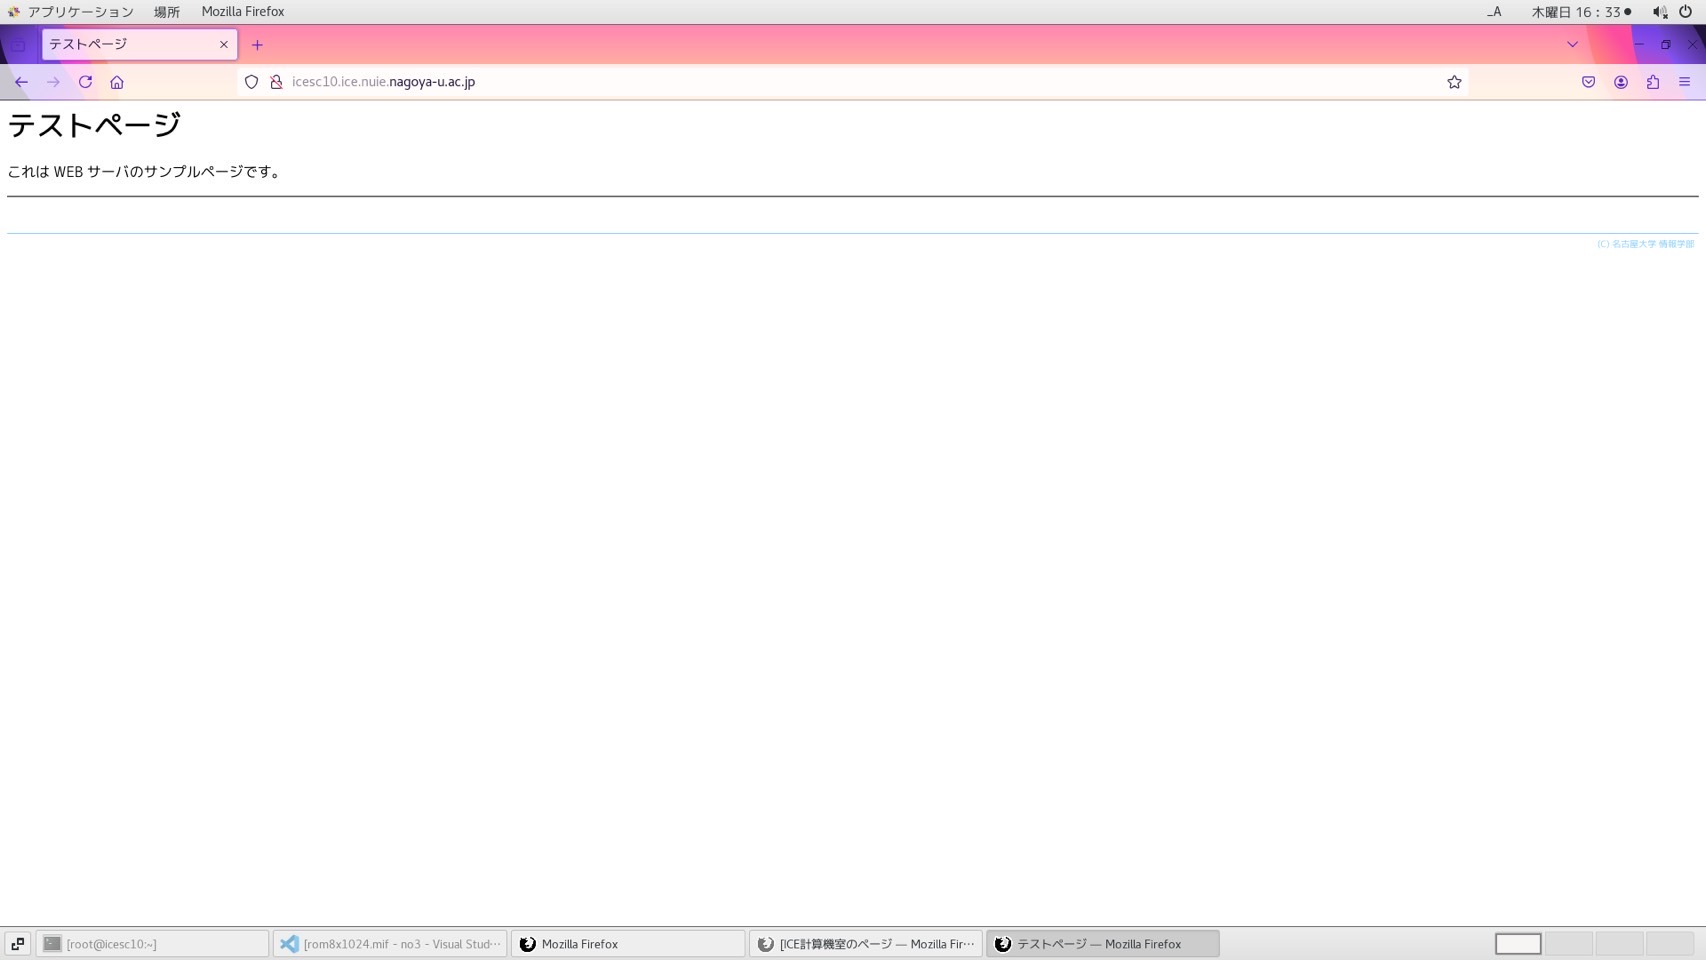
\includegraphics[width=1.0\textwidth]{http.JPEG} % 画像を挿入、幅をページ幅に合わせる
  \caption{httpの動作確認} % キャプションを追加
  \label{fig:http} % ラベルを追加
\end{figure}

\begin{figure}[H] % 画像を挿入する環境を開始
  \centering
  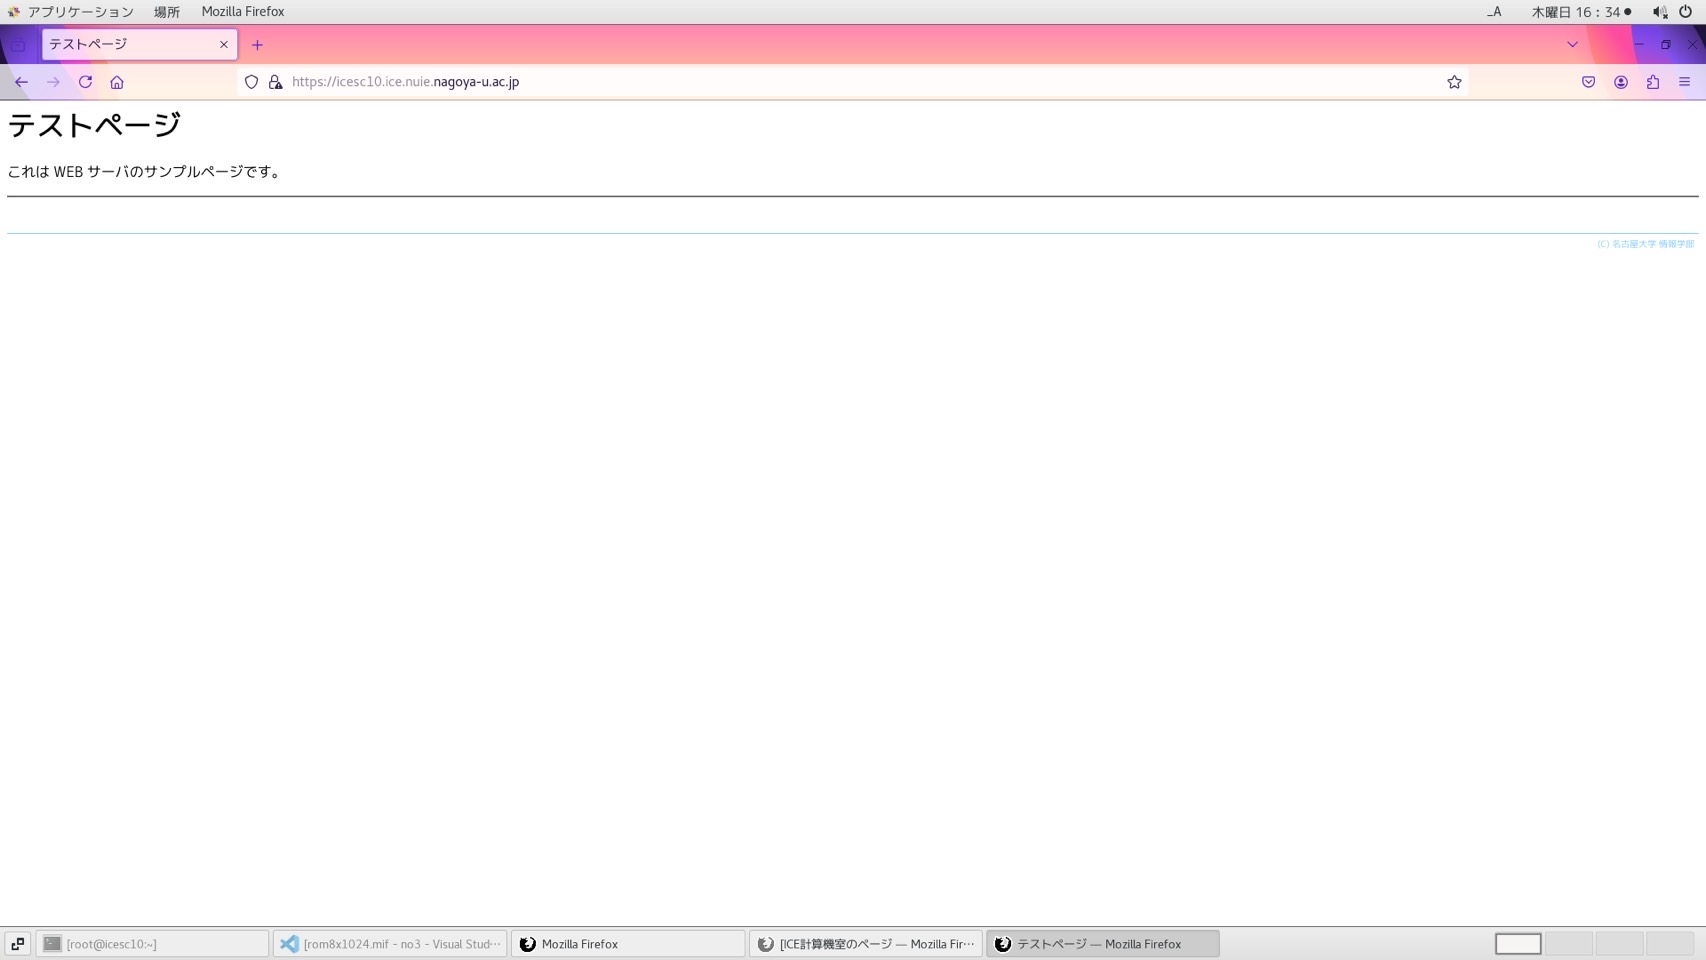
\includegraphics[width=1.0\textwidth]{https.JPEG} % 画像を挿入、幅をページ幅に合わせる
  \caption{httpsの動作確認} % キャプションを追加
  \label{fig:https} % ラベルを追加
\end{figure}

\subsection{考察}

\subsubsection{SSL/TLS 自己署名証明書の作成}
SSL/TLS, 自己署名証明書について調査した. 

SSL/TLS証明書は, インターネット上での安全な通信を保証するために使用される. 
証明書により, 通信が暗号化され, サーバーとクライアント間のデータの盗聴や改竄を防ぐことができる. 
また, 証明書には公開鍵が含まれ, 通信の安全性を確保することができる. 
(cybertrust, 2009)

自己署名証明書は, 認証局(CA)を介さずに, 個人または組織が自分で証明書を生成し, 署名したものである. 
自己署名証明書は, 本番環境での商用利用には向いていないが, 
内部システムや開発環境, テスト環境で使用される. 
例えば, 社内でのシステム間通信や開発中のアプリケーションにおいて, 自己署名証明書は有効である. 
(e-words, 2021)


\subsubsection{動作確認}
machine3に SSH 接続し, 「lynx 192.168.150.2」を実行した結果, 設定した WEB ページに接続することができたことから, 
machine3 から machine2 へ正常にネットワーク的に接続されており, DMZネットワークやファイアウォールの設定が正しく, 
HTTP通信が許可されている状態であると考えられる. 

ICE 端末から, firefox を用いて,「http://icesc10.ice.nuie.nagoya-u.ac.jp」に接続した結果, 設定した WEB ページが閲覧できたことから, 
外部端末から machine2 への DMZネットワークやファイアウォールの設定が正しく, HTTP通信が許可されている状態であると考えられる. 
また, ICE 端末から, firefox を用いて,「https://icesc10.ice.nuie.nagoya-u.ac.jp」に接続した結果, 設定した WEB ページが閲覧できたことから, 
外部端末から machine2 への HTTPS通信が許可されている状態であると考えられる. 

これらのことから machine2 の WWW サーバは正しく起動できたと考えられる. 


\section{まとめ}

\subsection{実験を通して分かったこと}
TCP/IP ネットワークにおける各種サービスの提供・利用のために必要な基本的知識を身に着けることができた. 

\subsection{工夫したこと}
実験で行ったことについて逐一メモや写真に記録を残し, 後から確認しやすいようにした. 

\subsection{反省点}
script コマンドで結果を保存する際に、行が切れてしまうことがあった. 
リダイレクトなどを使い結果をテキストファイルに保存するべきだった. 


\begin{thebibliography}{99} % 最大ラベル幅を99に設定
    
  \bibitem{lamport1994latex}
  syui: 
  \emph{iptablesを使いこなす}. \\
  \verb|https://qiita.com/syui/items/27020b970775a0c508ba|  2021. 
  \bibitem{lamport1994latex}
  cybertrust: 
  \emph{SSL/TLS サーバー証明書の基礎知識}. \\
  \verb|https://www.cybertrust.co.jp/blog/ssl/knowledge/ssl-basics.html|  2009.
  \bibitem{lamport1994latex}
  e-words: 
  \emph{自己署名証明書}. \\
  \verb|https://e-words.jp/w/自己署名証明書.html|  2021.

\end{thebibliography}


\end{document}